\part{UE4 Material System}
\frame{\partpage}

\begin{frame}{Shaders \& Game Engines}
\begin{itemize}
	\item Most Game Engines abstract shaders into Materials
	\pause\item These materials encapsulate a series of shaders and any other rendering states required to draw the effect
	\pause \item These systems allow greater control for performance
	\pause \item In addition, materials fit onto an Artists workflow
\end{itemize}
\end{frame}

\begin{frame}{UE4 Material System}
		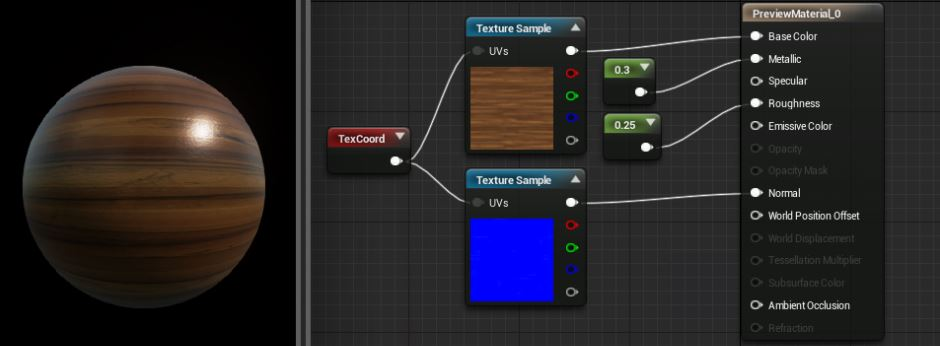
\includegraphics[height=0.8\textheight, width=1.0\textwidth]{UE4_material}
\end{frame}

\begin{frame}{UE4 Material System}
\begin{itemize}
	\item This system uses a visual programming language to control the look of an object in the scene
	\pause \item It consists of nodes called \textbf{Material Expressions}
	\pause \item These nodes are simply bits of shader code designed to perform a single task
	\begin{itemize}
		\item Multiplication
		\item Texture Sample (also know as a look up)
		\item Blends
	\end{itemize}
	\pause \item This allows you to build up a complex effect by chaining nodes together
\end{itemize}
\end{frame}

